\section{Introduction}

Le système de Thorlabs doit être utilisé par deux applications distinctes, Kinesis et ThorCam, pour être fonctionnel à 100\%. De ce fait, cela rends son utilisation moins ergonomique. De plus, de nombreuses fonctionnalités ont été implémentées par Thorlabs, aussi bien dans les logiciels Kinesis que ThorCam qui ne sont pas forcément utilisés dans les manipulations. Cela alourdit leur compréhension. Pour une manipulation de laboratoire, il est actuellement nécessaire d'avoir une notice très détaillée pour bien comprendre le fonctionnement du système, installer les logiciels et les configurer. Ce premier point va mener au premier objectif de cette nouvelle application.

Dans l'application Kinesis, aucun système de vision n'est intégrée et de ce fait, il est impossible de détecter automatiquement des particules. Ce second point va mener au deuxième objectif.

\section{Objectifs}
\begin{itemize}[label=\textbullet]
    \item Création de l'application ServoVision qui regroupent les fonctionnalités de base de Kinesis et de ThorCam afin d'avoir qu'une seule application simple d'utilisation. Le nom ServoVision vient de la combinaison de "Servo" pour la gestion des servomoteurs, et "Vision" pour le contrôle de la caméra.
    \item Intégration d'un algorithme pour détecter automatiquement des particules, et de les déplacer de façon autonome.
\end{itemize}

\newpage
\begin{minipage}{\textwidth}
    Ci-dessous, un tableau récapitulatif pour les fonctionnalités reprogrammées dans ServoVision :

    \begin{table}[H]
        \centering
        \begin{tabular}{|p{6cm}|c|c|c|}
            \hline
            \textbf{Fonctionnalité}                        & \textbf{Kinesis} & \textbf{ThorCam} & \textbf{ServoVision} \\
            \hline
            Contrôle des servomoteurs X et Y               & \ding{51}        &                  & \ding{51}            \\
            Contrôle du driver laser                       & \ding{51}        &                  & \ding{51}            \\
            \hline
            Affichage en direct de la caméra               &                  & \ding{51}        & \ding{51}            \\
            Pause / Play du flux caméra                    &                  & \ding{51}        & \ding{51}            \\
            Capture d'image                                &                  & \ding{51}        & \ding{51}            \\
            Enregistrement vidéo                           &                  & \ding{51}        & \ding{51}            \\
            Outils de mesure dans l'image                  &                  & \ding{51}        & \ding{51}            \\
            Zoom caméra                                    &                  & \ding{51}        & \ding{51}            \\
            Navigation caméra                              &                  & \ding{51}        & \ding{51}            \\
            \hline
            {\small Détection automatique de particules}   &                  &                  & \ding{51}            \\
            {\small Déplacement automatique de particules} &                  &                  & \ding{51}            \\
            \hline
        \end{tabular}
        \caption{Fonctionnalités reprogrammées de Kinesis et ThorCam dans l'application ServoVision}
        \label{tab:fonctionnalites_servovision}
    \end{table}
\end{minipage}
\newpage
\section{Choix des solutions}
Thorlabs met à disposition plusieurs outils pour développer sa propre application. Le logiciel Kinesis propose des contrôles .NET utilisables avec des langages comme C\#, Visual Basic, LabVIEW, ou tout autre langage compatible .NET. Des bibliothèques DLL bas niveau sont aussi disponibles. Les langages C, C++ et Python sont également compatible avec le matériel Thorlabs.

Du côté de ThorCam, un SDK (Software Development Kit) est fourni pour développer notre propre interface. Un SDK est un kit fourni par une entreprise qui contient tout le nécessaire (bibliothèques, exemples, docs) pour créer sa propre application. Il est également possible d'utiliser les langages de programmation: C\#, C++, MATLAB et Python.

Grâce à ces bibliothèques et outils, il est donc possible de regrouper les fonctions essentielles de Kinesis et ThorCam dans une seule application personnalisée.
\subsection{Choix du language de programmation}
\begin{table}[H]
    \centering
    \begin{tabular}{|l|c|c|c|c|c|}
        \hline
        \textbf{Critère}                  & \textbf{C\#} & \textbf{C++} & \textbf{Python} & \textbf{MATLAB} & \textbf{LabVIEW} \\
        \hline
        Compatibilité driver moteur       & 6            & 6            & 6               & 6               & 4                \\
        Compatibilité driver laser        & 6            & 6            & 2               & 6               & 2                \\
        Compatibilité caméra              & 6            & 6            & 6               & 6               & 6                \\
        Intégration interface utilisateur & 6            & 4            & 4               & 2               & 2                \\
        Documentation Thorlabs            & 6            & 6            & 4               & 4               & 4                \\
        Facilité de programmation         & 5            & 4            & 5               & 5               & 6                \\
        Multi-plateforme                  & 3            & 5            & 6               & 4               & 4                \\
        Évolutivité                       & 6            & 5            & 5               & 3               & 2                \\
        Modularité                        & 6            & 5            & 5               & 3               & 2                \\
        Organisation du code              & 6            & 5            & 5               & 3               & 2                \\
        \hline
        \textbf{Note moyenne}             & \textbf{5.6} & \textbf{5.2} & \textbf{4.8}    & \textbf{4.2}    & \textbf{3.4}     \\
        \hline
    \end{tabular}
    \caption{Évaluation des langages pour l'application ServoVision (6 = excellent, 1 = faible)}
    \label{tab:langages}
\end{table}
Le tableau~\ref{tab:langages} est composé de critères importants pour l'application. Il en ressort que le C\# est le plus adapté à ce projet. Ce langage permet de créer une interface graphique complète grâce au framework WPF (Windows Presentation Foundation), qui offre une grande flexibilité dans la création d'interfaces modernes. L'organisation claire du code ainsi que sa modularité font de C\# un choix idéal pour une application évolutive et maintenable.

Python est LabVIEW ont obtenu la note de 2 pour la compatibilité avec le driver laser, car Thorlabs n'ont pas d'exemples sur leur github pour cet appareil, mais il faudrait utiliser d'autres librairies supplémentaires~\cite{controlLaserDriverPython}~\cite{controlLaserDriverLabVIEW}.

\newpage
\subsection{Architecture logicielle}
Ci-dessous, le diagramme UML met en évidence les différentes classes principales et leurs relations entre elles.
\begin{figure}[H]
    \centering
    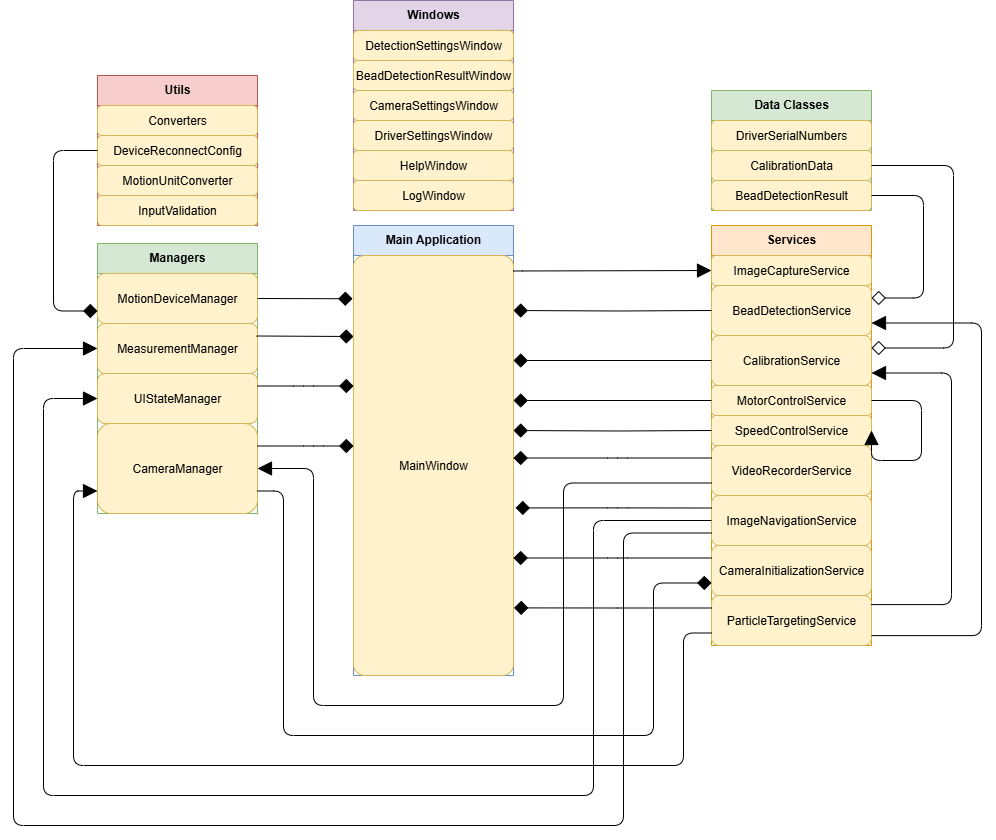
\includegraphics[width=\textwidth]{assets/figures/Application_ServoVision/ServoVision_UML_Diagram.drawio.png}
    \caption{Diagramme UML de l'architecture logicielle de l'application ServoVision}
    \label{uml_servovision}
\end{figure}

Seuls les services sont expliqués ici, car ce sont les principales classes permettant de comprendre le fonctionnement du code. Les différentes fenêtres sont présentées à l'aide de captures d'écran provenant de l'application à la section~\ref{subsection:fenetres}.

\textbf{CalibrationService}
\begin{itemize}[label=\textbullet]
    \item Calibration pour faire correspondre les pas du moteur avec l'image à la caméra
    \item Calcul des facteurs de conversion pixel/mm
\end{itemize}

\textbf{CameraInitializationService}
\begin{itemize}[label=\textbullet]
    \item Détection automatique des caméras Thorlabs
    \item Gestion des erreurs de connexion
\end{itemize}

\textbf{MotorControlService}
\begin{itemize}[label=\textbullet]
    \item Contrôle en temps réel des moteurs X/Y
    \item Contrôle de la vitesse de déplacement
    \item Interface avec le clavier pour les mouvements
\end{itemize}

\textbf{SpeedControlService}
\begin{itemize}[label=\textbullet]
    \item Gestion de la vitesse de déplacement des moteurs
    \item Interface avec les contrôles de vitesse
\end{itemize}

\textbf{ImageNavigationService}
\begin{itemize}[label=\textbullet]
    \item Zoom et dézoom de l'image
    \item Déplacement dans l'image
    \item Gestion des interactions souris
\end{itemize}

\textbf{BeadDetectionService}
\begin{itemize}[label=\textbullet]
    \item Algorithme de détection basé sur OpenCV
    \item Seuillage adaptatif pour avoir une image binaire
    \item Filtrage par taille des objets détectés
\end{itemize}

\textbf{ParticleTargetingService}
\begin{itemize}[label=\textbullet]
    \item Sélection de particules par clic
    \item Calcul des mouvements moteur nécessaires
    \item Compensation du jeu mécanique
    \item Mouvement automatique vers la particule sélectionnée
\end{itemize}

\textbf{ImageCaptureService}
\begin{itemize}[label=\textbullet]
    \item Capture d'images individuelles
    \item Organisation des fichiers par date/heure
    \item Interface utilisateur pour la sélection du dossier
\end{itemize}

\textbf{VideoRecorderService}
\begin{itemize}[label=\textbullet]
    \item Enregistrement vidéo en temps réel
    \item Sauvegarde automatique des vidéos
\end{itemize}

\newpage
\subsection{Présentation de l'application} \label{subsection:fenetres}
\subsubsection{Moteurs X / Y, Laser et calibration}

\begin{figure}[H]
    \centering
    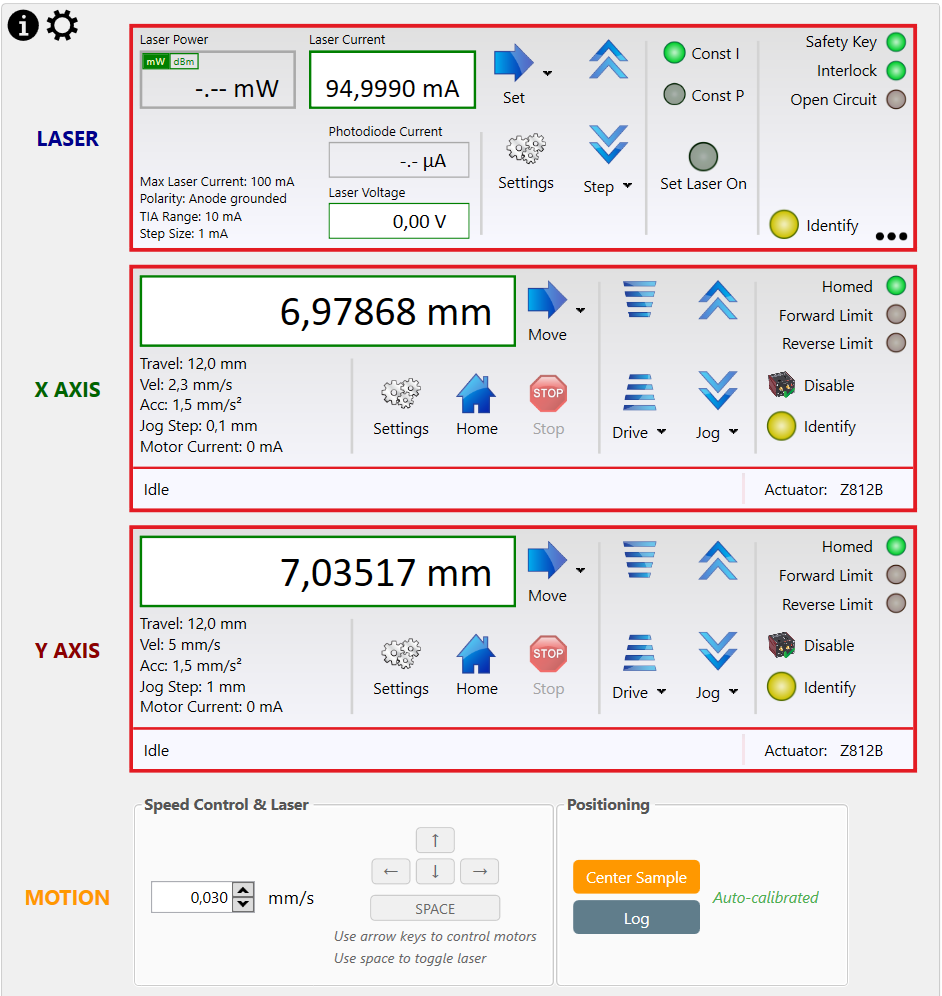
\includegraphics[width=\textwidth]{assets/figures/Application_ServoVision/Moteurs_Laser_Calibration.png}
    \caption{Interface de contrôle des moteurs, du laser et de la calibration}
    \label{Moteurs_Laser_Calibration}
\end{figure}
Cette partie de l'application permet de gérer les moteurs, le laser et la calibration. On peut voir que les trois drivers reprennent exactement le même visuel que dans Kinesis. La bibliothèque fournie par Thorlabs permet d'intégrer directement leurs modules dans une application personnalisée. C'est un point positif, car je n'ai pas eu à reprogrammer tous les boutons de ces drivers.

Dans l'onglet \textcolor[RGB]{241,158,56}{\textbf{MOTION}} il y'a deux sous-groupes, le premier est \textbf{Speed Control \& Laser}, il permet de choisir la vitesse en mm/s souhaitée, puis il suffit d'utiliser les touches du clavier pour se déplacer. Pour un confort optimal, l'appui sur la touche espace permet d'activer/désactiver le laser.

\newpage
Dans le deuxième sous-groupe \textbf{Positioning}, on retrouve le premier bouton \textcolor[RGB]{241,158,56}{\textbf{Center Sample}} qui permet de centrer l'échantillon sous le microscope, ce qui correspond à un déplacement des axes X et Y à 7mm sur chacun d'eux.

Le bouton \textcolor[RGB]{102,125,138}{\textbf{Log}} affiche les logs de la calibration~(Figure~\ref{Calibration_Center_logs}).
\begin{figure}[H]
    \centering
    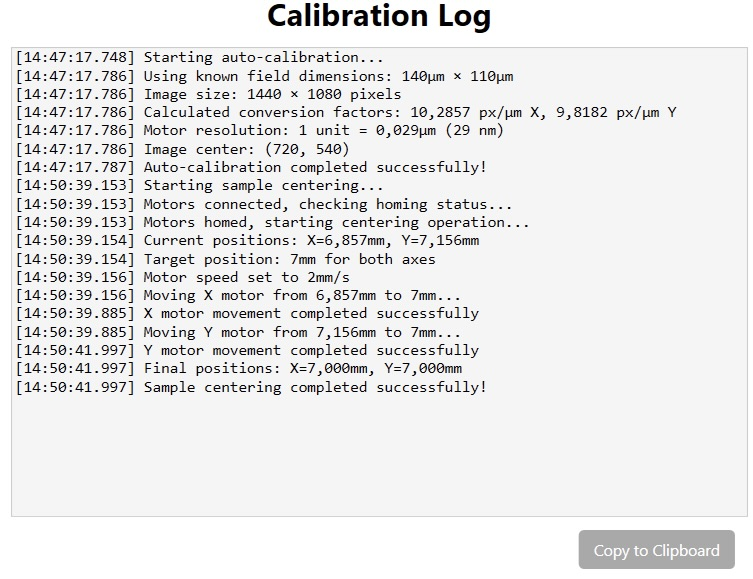
\includegraphics[width=0.8\textwidth]{assets/figures/Application_ServoVision/Calibration_Center_logs.jpeg}
    \caption{Calibration avec sa journalisation}
    \label{Calibration_Center_logs}
\end{figure}
Cette calibration consiste à calculer combien il y a de pixels pour 1~\textmu m dans l'image de la caméra, pour ensuite savoir de combien doit se déplacer un moteur pour parcourir une certaine distance en unité réelle.

Pour connaître la taille du champ observé, je place un point fixe sur un bord de l'image, puise je me déplace jusqu'à ce que ce même point soit de l'autre côté. Je peux ensuite observer l'écart affiché par le servomoteur. Je fais la même procédure pour l'autre dimension.

Connaissant la résolution de l'image capturée par la caméra et la taille du champ observé en \textmu m, on peut calculer un facteur de conversion en X et en Y.

Dans notre cas:
\begin{itemize}
    \item Image : 1440~$\times$~1080 pixels (section 5.1 du manuel de la caméra~\cite{cameraCS165CU/M})
    \item Champ de la caméra : 140~\textmu m~$\times$~110~\textmu m
\end{itemize}

Les équations des facteurs de calibration en X et Y sont :

\[
    \text{Facteur}_X = \frac{1440\ \text{pixels}}{140\ \mu m} = 10.29\ \text{pixels}/\mu m
\]
\[
    \text{Facteur}_Y = \frac{1080\ \text{pixels}}{110\ \mu m} = 9.82\ \text{pixels}/\mu m
\]

On connaît aussi le pas des moteurs de la table du microscope utilisé : 1~pas~=~29~nm (section 5.2 du manuel des moteurs~\cite{motorZ812B}). Grâce à ça, on peut directement relier un déplacement moteur à une distance réelle. À l'aide des facteurs de calibration pixels/\textmu m, ça permet un positionnement précis basé sur l'image de la caméra.

\subsubsection{Réglage numéros de série des drivers}

\begin{minipage}[c]{0.4\textwidth}
    En cliquant sur la roue dentée en haut à gauche (Figure~\ref{Moteurs_Laser_Calibration}), il est possible de modifier les numéros de séries de chaque driver. La connexion de nouveaux appareils se fait automatiquement. Un bouton reset est présent afin de remettre les numéros de séries par défaut des appareils. Ces numéros sont montrés dans la figure~\ref{Settings_Drivers}.
\end{minipage}
\begin{minipage}[c]{0.58\textwidth}
    \begin{center}
        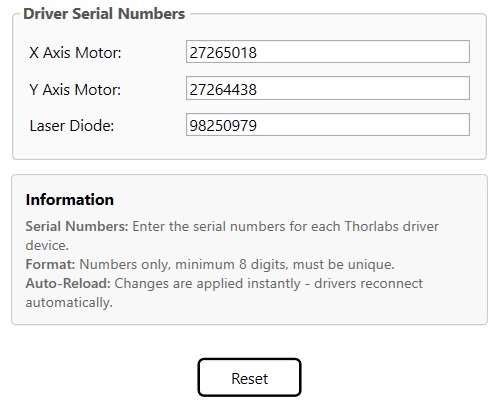
\includegraphics[width=\textwidth]{assets/figures/Application_ServoVision/Settings_Drivers.png}
    \end{center}
    \captionof{figure}{Configuration des numéros de série des drivers}
    \label{Settings_Drivers}
\end{minipage}

\subsubsection{Caméra, outil de mesure, capture d'écran}

\begin{figure}[H]
    \centering
    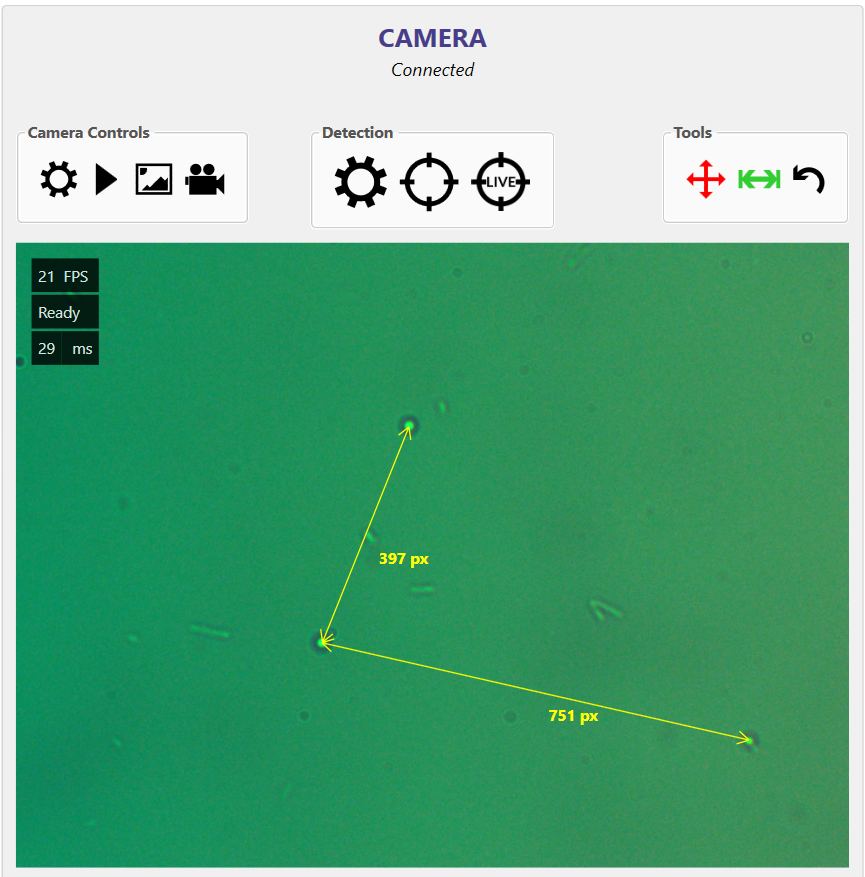
\includegraphics[width=0.7\textwidth]{assets/figures/Application_ServoVision/Measure_Tool.png}
    \caption{Interface de contrôle de la caméra}
    \label{Measure_Tool}
\end{figure}
La partie de droite de l'application concerne l'interface de la caméra. Au centre de l'image, on aperçoit le retour visuel de la caméra. Deux sous-groupes vont être détaillés ici.
\newpage
Le premier sous-groupe \textbf{Camera Controls}, permet la gestion visuelle de l'image, on y retrouve :
\begin{itemize}[label=\textbullet]
    \item Le bouton \textbf{PLAY} met en pause l'image.
    \item Le bouton avec une \textbf{image de paysage} permet de faire une capture d'écran de l'image en cours.
    \item Le bouton \textbf{Camera} enregistre une vidéo de l'image en cours.
    \item
          \begin{minipage}{0.4\textwidth}
              Le bouton \textbf{Réglages} ouvre les paramètres de la caméra (Figure~\ref{Settings_Camera}) où l'on va pouvoir modifier les gains de couleurs sur le rouge, vert et bleu. Le temps d'exposition est également un paramètre qui peut être réglé.
          \end{minipage}
          \hfill
          \begin{minipage}{0.55\textwidth}
              \centering
              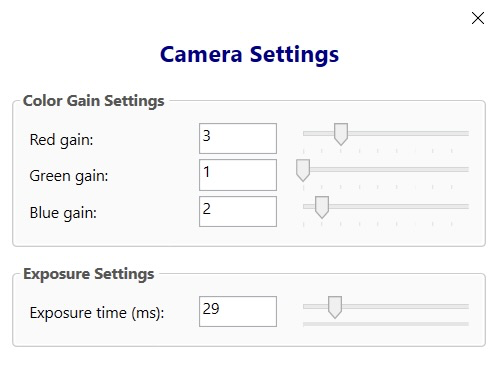
\includegraphics[width=\textwidth]{assets/figures/Application_ServoVision/Settings_Camera.png}
              \captionof{figure}{Réglages de la caméra}
              \label{Settings_Camera}
          \end{minipage}
\end{itemize}
Le sous-groupe \textbf{Tools} contient trois boutons :
\begin{itemize}[label=\textbullet]
    \item La première fonctionnalité qui n'est pas représentée par un bouton est le zoom. Avec la molette de la souris, il est possible de zoomer et de dézoomer dans l'image.
    \item Le premier bouton représenté par quatres flèches permet de se déplacer dans l'image une fois zoomé à l'intérieur.
    \item Le deuxième bouton, avec deux flèches, est un outil de mesure. Il permet de mesurer en pixels la distance entre deux points de l'image. Lors de l'affichage, des flèches jaunes sont dessinées avec la dimension en pixels indiquée à côté (Figure~\ref{Measure_Tool}).
    \item Le dernier bouton avec une flèche incurvée permet de supprimer la dernière flèche dessinée.
\end{itemize}

\newpage
\subsubsection{Détection automatique de particules avec adaptative threshold}
Le dernier sous-groupe \textbf{Detection} va regrouper toutes les fonctionnalités par rapport à la détection de particules. Le premier bouton \textbf{Réglage} va être détaillé avec la Figure~\ref{Settings_Detection}.
\begin{figure}[H]
    \centering
    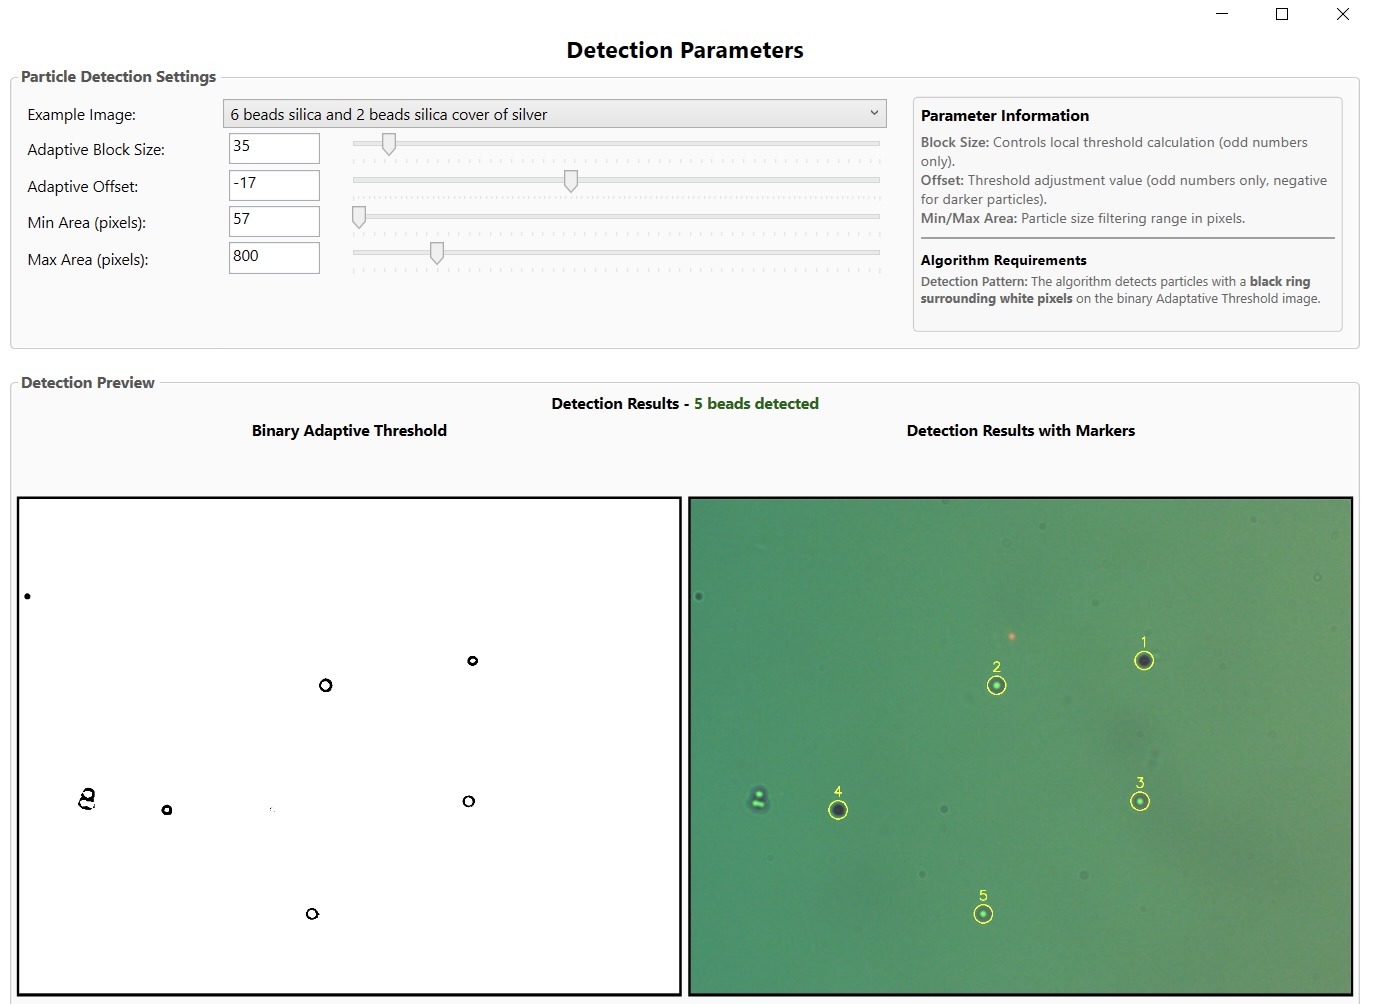
\includegraphics[width=0.9\textwidth]{assets/figures/Application_ServoVision/Settings_Detection.jpeg}
    \caption{Réglages de la détection des particules, les particules numérotées sont celles détectées par l'algorithme}
    \label{Settings_Detection}
\end{figure}
Le premier sous-groupe, \textbf{Particle Detection Settings}, permet de gérer les différents paramètres pour la détection de particules.

L'algorithme principal utilisé pour cette détection est l'\textit{adaptive threshold} de la bibliothèque OpenCV. L'adaptive thresholding calcule un seuil différent pour chaque pixel en fonction de l'intensité locale dans une région définie par le paramètre  \textit{block size} (taille du voisinage). Le seuil est ajusté en soustrayant une valeur constante appelée \textit{offset}, ce qui permet d'affiner la sensibilité du seuillage~\cite{OpenCVadaptativeThreshold}.
\newpage
\begin{figure}[H]
    \centering
    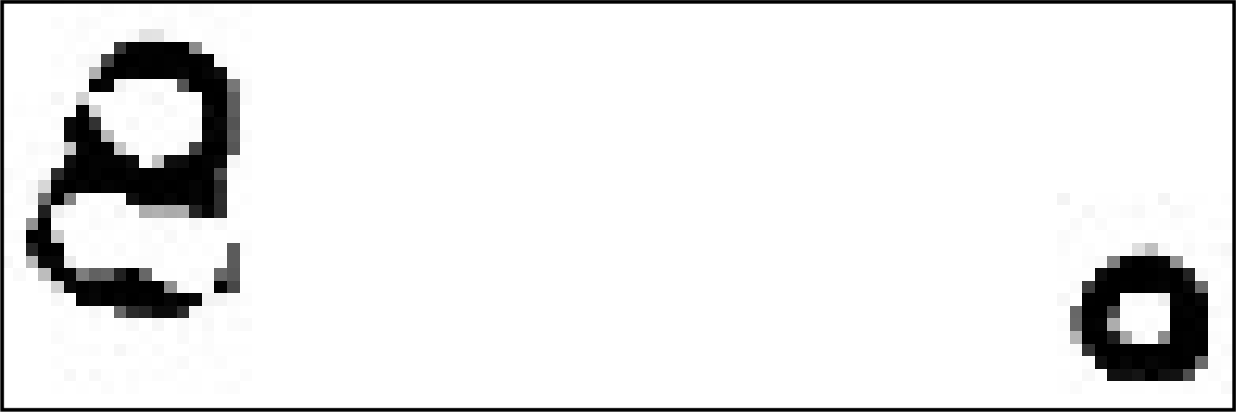
\includegraphics[width=0.9\textwidth]{assets/figures/Application_ServoVision/Settings_Detection_zoom.png}
    \caption{Zoom sur l'image noir et blanc \textit{Binary Adaptive Threshold} de la figure~\ref{Settings_Detection}}
    \label{Settings_Camera_zoom}
\end{figure}

L'algorithme fonctionne seulement si un anneau de pixels éteints (noirs) est fermé. On peut voir sur la figure~\ref{Settings_Camera_zoom}, l'anneau noir à droite sera considéré comme une particule, et à gauche non car ce n'est pas fermé.

Au moment de dire si oui ou non une zone de l'image est considérée comme une particule, la plus grande zone de pixels allumés (blancs) est retirée, car elle correspond au fond blanc de l'image. Découlant de cette opération, si un anneau de pixels éteint n'est pas complétement fermé, il sera intégré à cette grande forme et ne sera pas identifié comme une vraie particule.

Ensuite, il suffit d'énumérer les zones blanches restantes (donc l'intérieur des anneaux noirs fermés) qui sont des particules.

On peut définir l'aire minimale et maximale, en pixels, qu'une région blanche doit avoir pour être considérée comme une particule.

Une série d'images tests est disponible à l'utilisateur pour qu'il puisse essayer différents paramètres.

Toujours dans le sous-groupe \textbf{Detection}, le bouton au milieu avec une \textbf{cible}, lance une détection de particules sur une image capturée. Le même bouton, mais avec le mot \textbf{LIVE} en son centre, lance également une détection de particules, mais cette fois en temps réel.
\newpage
\begin{figure}[H]
    \centering
    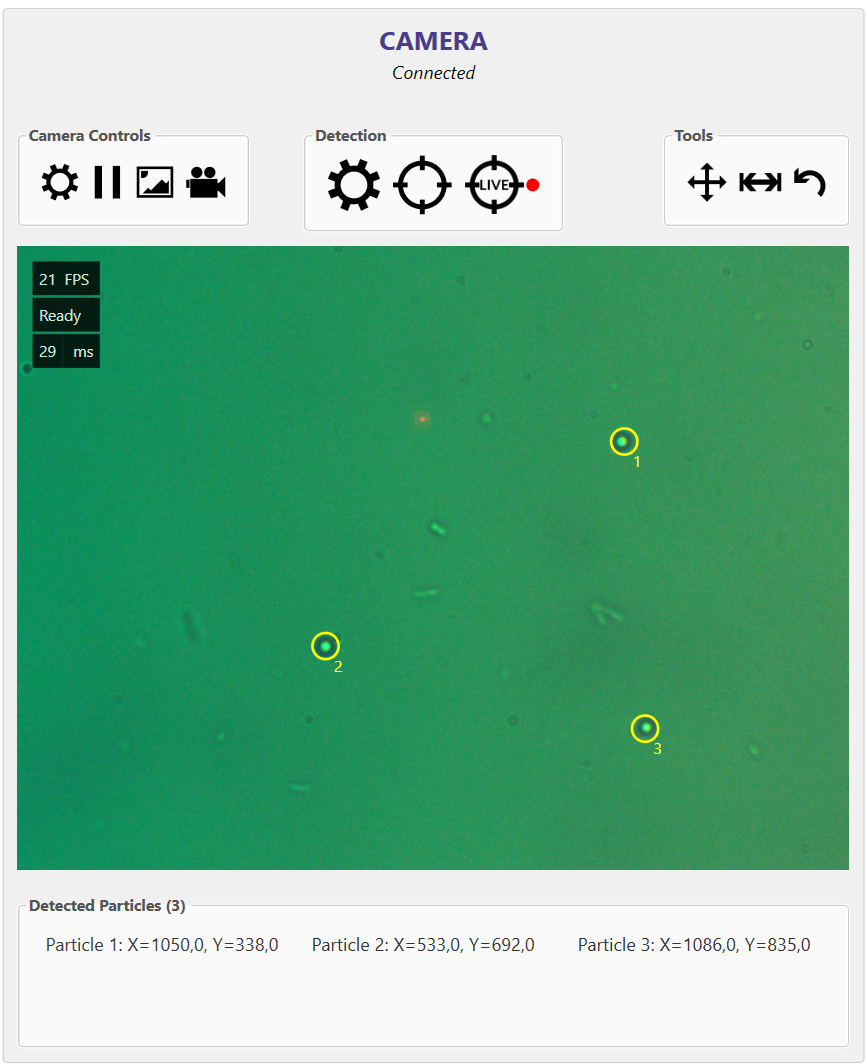
\includegraphics[width=\textwidth]{assets/figures/Application_ServoVision/Live_Targeting_Bead.png}
    \caption{Détection de particules en temps réel}
    \label{Live_Targeting_Bead}
\end{figure}

Dans le sous-groupe \textbf{Detected Particles} de la Figure~\ref{Live_Targeting_Bead}, il est possible de visualiser la liste des particules détectées, avec leur coordonnées et un numéro attribué à chacune d'elles. Les coordonnées en X se lisent de gauche à droite, et pour celles en Y de haut en bas.

\newpage
\subsubsection{Déplacement automatique de particules vers le laser}
Une dernière fonctionnalité au niveau de déplacement automatique de particules a été ajoutée. Si le système détecte une particule, l'utilisateur peut cliquer sur celle-ci dans la liste, et le système va amener cette particule choisie aux coordonnées du laser.

Comme première approche, on pourrait penser qu'il suffit de prendre les coordonnées de la particule sélectionnée, puis de déplacer les moteurs pour aligner le laser sur celle-ci. En réalité, c'est plus complexe que cela.

Un paramètre qui paraît anodin, mais qui a toute son importance à cette échelle, est le \textbf{jeu mécanique des moteurs}. En effet, lorsqu'on effectue un déplacement dans une direction, puis qu'on veuille repartir dans la direction opposée, il faut d'abord compenser ce jeu.

Pour les moteurs utilisés dans ce système (Z812B), la datasheet indique qu'il y a un jeu mécanique (\textit{backlash}) inférieur à 8~\textmu m (section 5.1 de la datasheet~\cite{motorZ812B}).

La procédure du déplacement de la particule sous le laser est décrite ci-dessous:
\begin{enumerate}
    \item Mouvements en X et Y de +8~\textmu m pour être sûr de corriger le jeu mécanique.
    \item Une nouvelle image est acquise et on cherche la particule la plus proche de la particule trouvée avant les déplacements, ce qui devrait donner la même particule, en supposant qu'elle n'a pas bougée. À présent, les vraies coordonnées de la particule sont acquises.
    \item Calcul de la distance à parcourir entre la particule et le laser.
    \item Déplacement vers le laser en X et en Y.
    \item
          La dernière étape consiste à rattraper une dernière fois le jeu mécanique. La Figure~\ref{schema_explicatif_jeu} illustre ce problème. Pour amener le laser sur la particule, appliquer simplement un déplacement en X et en Y ne suffit pas :  quatres cas différents risquent d'arriver.

          Si la particule se trouve dans le quadrant n\textsuperscript{o}1, le positionnement final sera juste. En revanche, si elle se situe dans un autre quadrant, il reste une dernière opération à effectuer.

          Vu que la compensation du jeu mécanique a été effectué dans les directions positives de chaque axe, un déplacement dans la direction opposée nécessitera de compenser à nouveau le jeu.

\end{enumerate}
\begin{figure}[H]
    \centering
    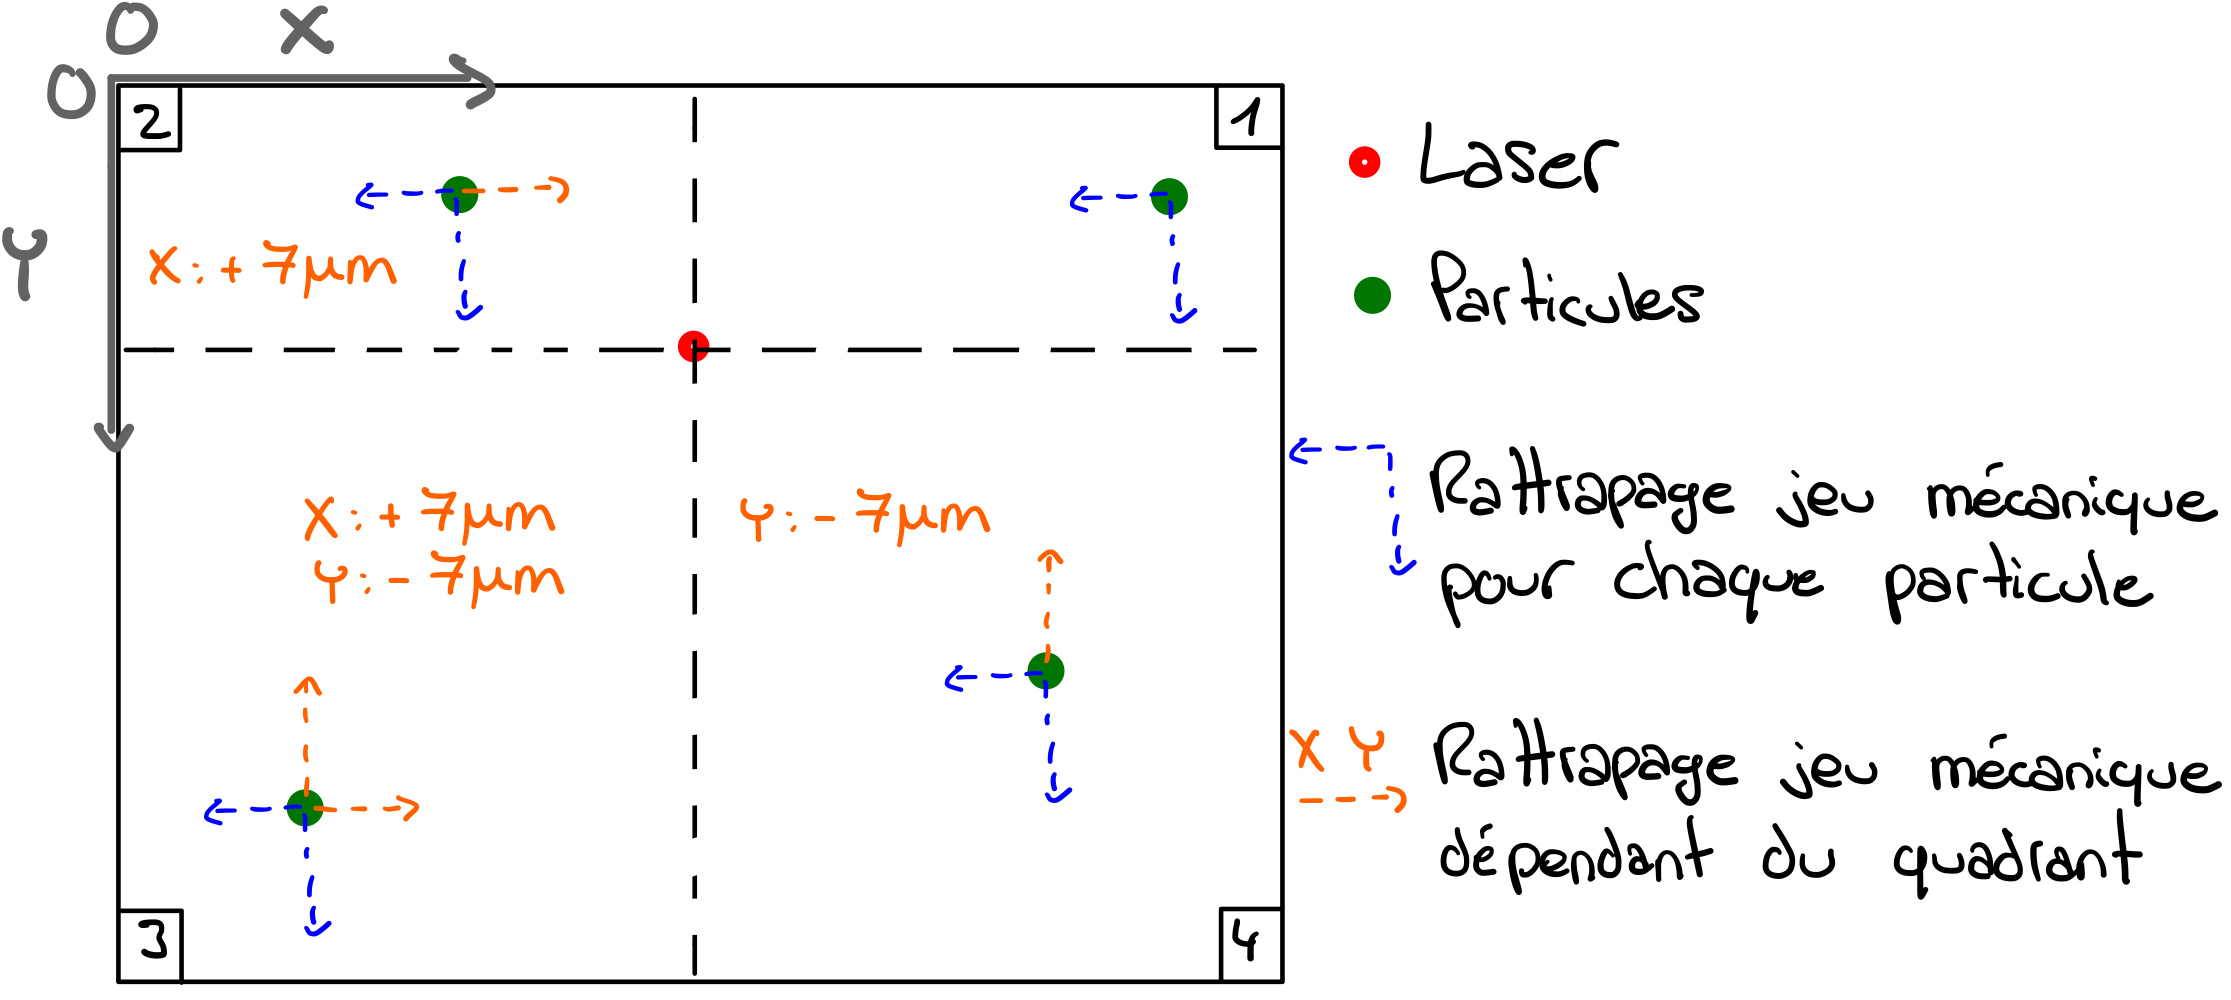
\includegraphics[width=0.9\textwidth]{assets/figures/Application_ServoVision/Schema_explicatif_jeu_mecanique.jpeg}
    \caption{Schéma explicatif pour la compensation du jeu mécanique des moteurs}
    \label{schema_explicatif_jeu}
\end{figure}

\subsubsection{Fiabilité et répétabilité de la détection et déplacement d'une particule}
\textbf{Fiabilité}

La fiabilité de la détection dépend pas mal des bons réglages à faire dans les paramètres (taille des particules, seuils, etc...). Si on prend le temps de bien les ajuster pour les conditions d'image qu'on a (bon contraste, particules bien visibles), la détection fonctionne bien. Une fois les bons paramètres trouvés, la particule est détectée presque à chaque fois, ce qui montre que la fiabilité est plutôt bonne.

\textbf{Répétabilité}

Tant que la position de la particule est bien connue et que la connexion avec les moteurs fonctionne, le déplacement jusqu'au laser se fait sans problème. Le système refait les mouvements de manière stable. Bien sûr, il peut y avoir un léger décalage à l'arrivée. Le plus gros écart que j'ai pu observer était d'environ 20 pixels.

En résumé, le système est fiable tant au niveau de la détection que du déplacement, à condition de bien régler les paramètres de base. Ça fonctionne bien dans la majorité des cas, avec une précision qui reste suffisante pour l'objectif visé.